\section{Encoding rigid body kinematics}
\label{sec:Representations}

We now set up the required notation. Without loss of generality, we explain this using an example from our application domain
(Figure~\ref{fig:Learning.setup1}). Three reference frames $A$, $B$
and $O$, sit in a $3$\nobreakdash-\hspace{0pt}dimensional Cartesian
space. Frame $A$ is attached to a robot finger, which pushes an object with frame $B$, which in turn is placed on a table top with frame
$O$.\footnote{Although it is an abuse of notation, we
  use $A$, $B$ and $O$ to denote both the frame and the bodies to which they attach.} While frame $O$ is fixed, $A$ and $B$ change in time and are observed at discrete time steps $..., t-1, t, t+1, ...$.  Frame $X$ at
time step $t$ is denoted $X_t$, and the rigid body transformation
from a frame $X$ to a frame $Y$ is denoted by $T^{X, Y}$.

From classical mechanics, we know that in order to predict the change
in state of a rigid body it is sufficient to know its mass, velocity,
and a net force applied to the body.  We do not assume any knowledge of
the mass and applied forces, learning only from object trajectories.\footnote{We could include forces, and sense them with a force/torque sensor. This is future work.} We can, however, use the motion of a body over time to encode acceleration---an effect of the applied net
force. We therefore use rigid body transformations, $T^{X,Y}$, of the interacting bodies through time (Figure~\ref{fig:Learning.setup1}). Given the additional assumption that the net force and the body mass are constant, two subsequent rigid body transformations, $T^{B_{t-1},
  B_{t}}$ and $T^{B_{t},B_{t+1}}$, give a complete description of the
state of some body B (here the object) at time step $t$, in the absence
of the other bodies.  Adding the transformation $T^{B_t, O}$, to give a
triple of transformations, thus provides a complete description of the
state of body B in the fixed frame $O$ (the stationary elements of the
environment).  Similarly, a second triple of transformations, $T^{A_t,
  O}$, $T^{A_{t-1}, A_{t}}$ and $T^{A_{t}, A_{t+1}}$, provides such a
description for some other body (here the finger) with frame $A$. 
The state of these two interacting bodies, with frames $A$, $B$ and the fixed environment $O$, can thus be adequately described by these six transformations.

In fact, we replace transformation $T^{A_t, O}$ by relative transformation $T^{A_t, B_t}$. This explicitly captures the spatial relationship, and thus any contacts, between $A$ (finger) and $B$ (object). This gives us a representation consisting of the set of six transformations marked in bold dotted lines in Figure~\ref{fig:Learning.setup1}. The general prediction problem is to predict the motion, $T^{B_t,B_{t+1}}$, of the object $B$ given these five transformations. In fact, in the experimental work described in this paper, we reduce the problem to a quasi-static one, relying only on transformations $T^{A_t,A_t+1}$, $T^{B_t,O}$, and $T^{A_t, B_t}$. This  dimensionality reduction makes learning easier.\footnote{It may be that other representations contain enough information to predict. To  avoid the quasi-static assumption it may be that finding a subspace in which the sets of transformation typically lie is a promising route.} Next, before defining the problem formally, we need to think briefly about how best to store these transformations.

Specifically, since we are interested in learning, we need to express this set of transformations in a way that supports generalised predictions. We make extensive use of transformations relative to the frame of the object about which predictions are made. Thus all transformations for learning are expressed in a frame attached to the body of the object, e.g. $T_{body}^{X_{t}, X_{t+1}}$. At prediction time these transformations are converted into a general inertial frame located in the world, thus becoming for example $T_{in}^{X_{t},X_{t+1}}$. 
%In general the behaviours of interacting bodies described by frames from Figure~\ref{fig:Learning.setup1} are independent of any inertial frame \citep{kopicki_prediction_2010}. Unfortunately, a na\"{\i}ve representation of transformation $T^{A_{t}, A_{t+1}}$ as $A_{t+1}(A_{t})^{-1}$, or explicitly given inertial frame $I$,
%% MAREK CHECK
%\begin{equation}
%T_{in}^{A_{t}, A_{t+1}} = T^{I, A_{t+1}} (T^{I, A_{t}})^{-1}
%\label{eq:Learning.In1}
%\end{equation}
%\noindent makes the transformation in \eqref{eq:Learning.In1} dependent on the currently used inertial frame $I$ (see
%Figure~\ref{fig:similarity}).  This would make the stored transformations poor from the point of view of generalisation. A better way is instead to store all the transformations in a body frame (at learning time) and convert to and from an inertial frame dependent transformation (at prediction time) using similarity transforms.
%
%\begin{figure}[b]
%\centerline{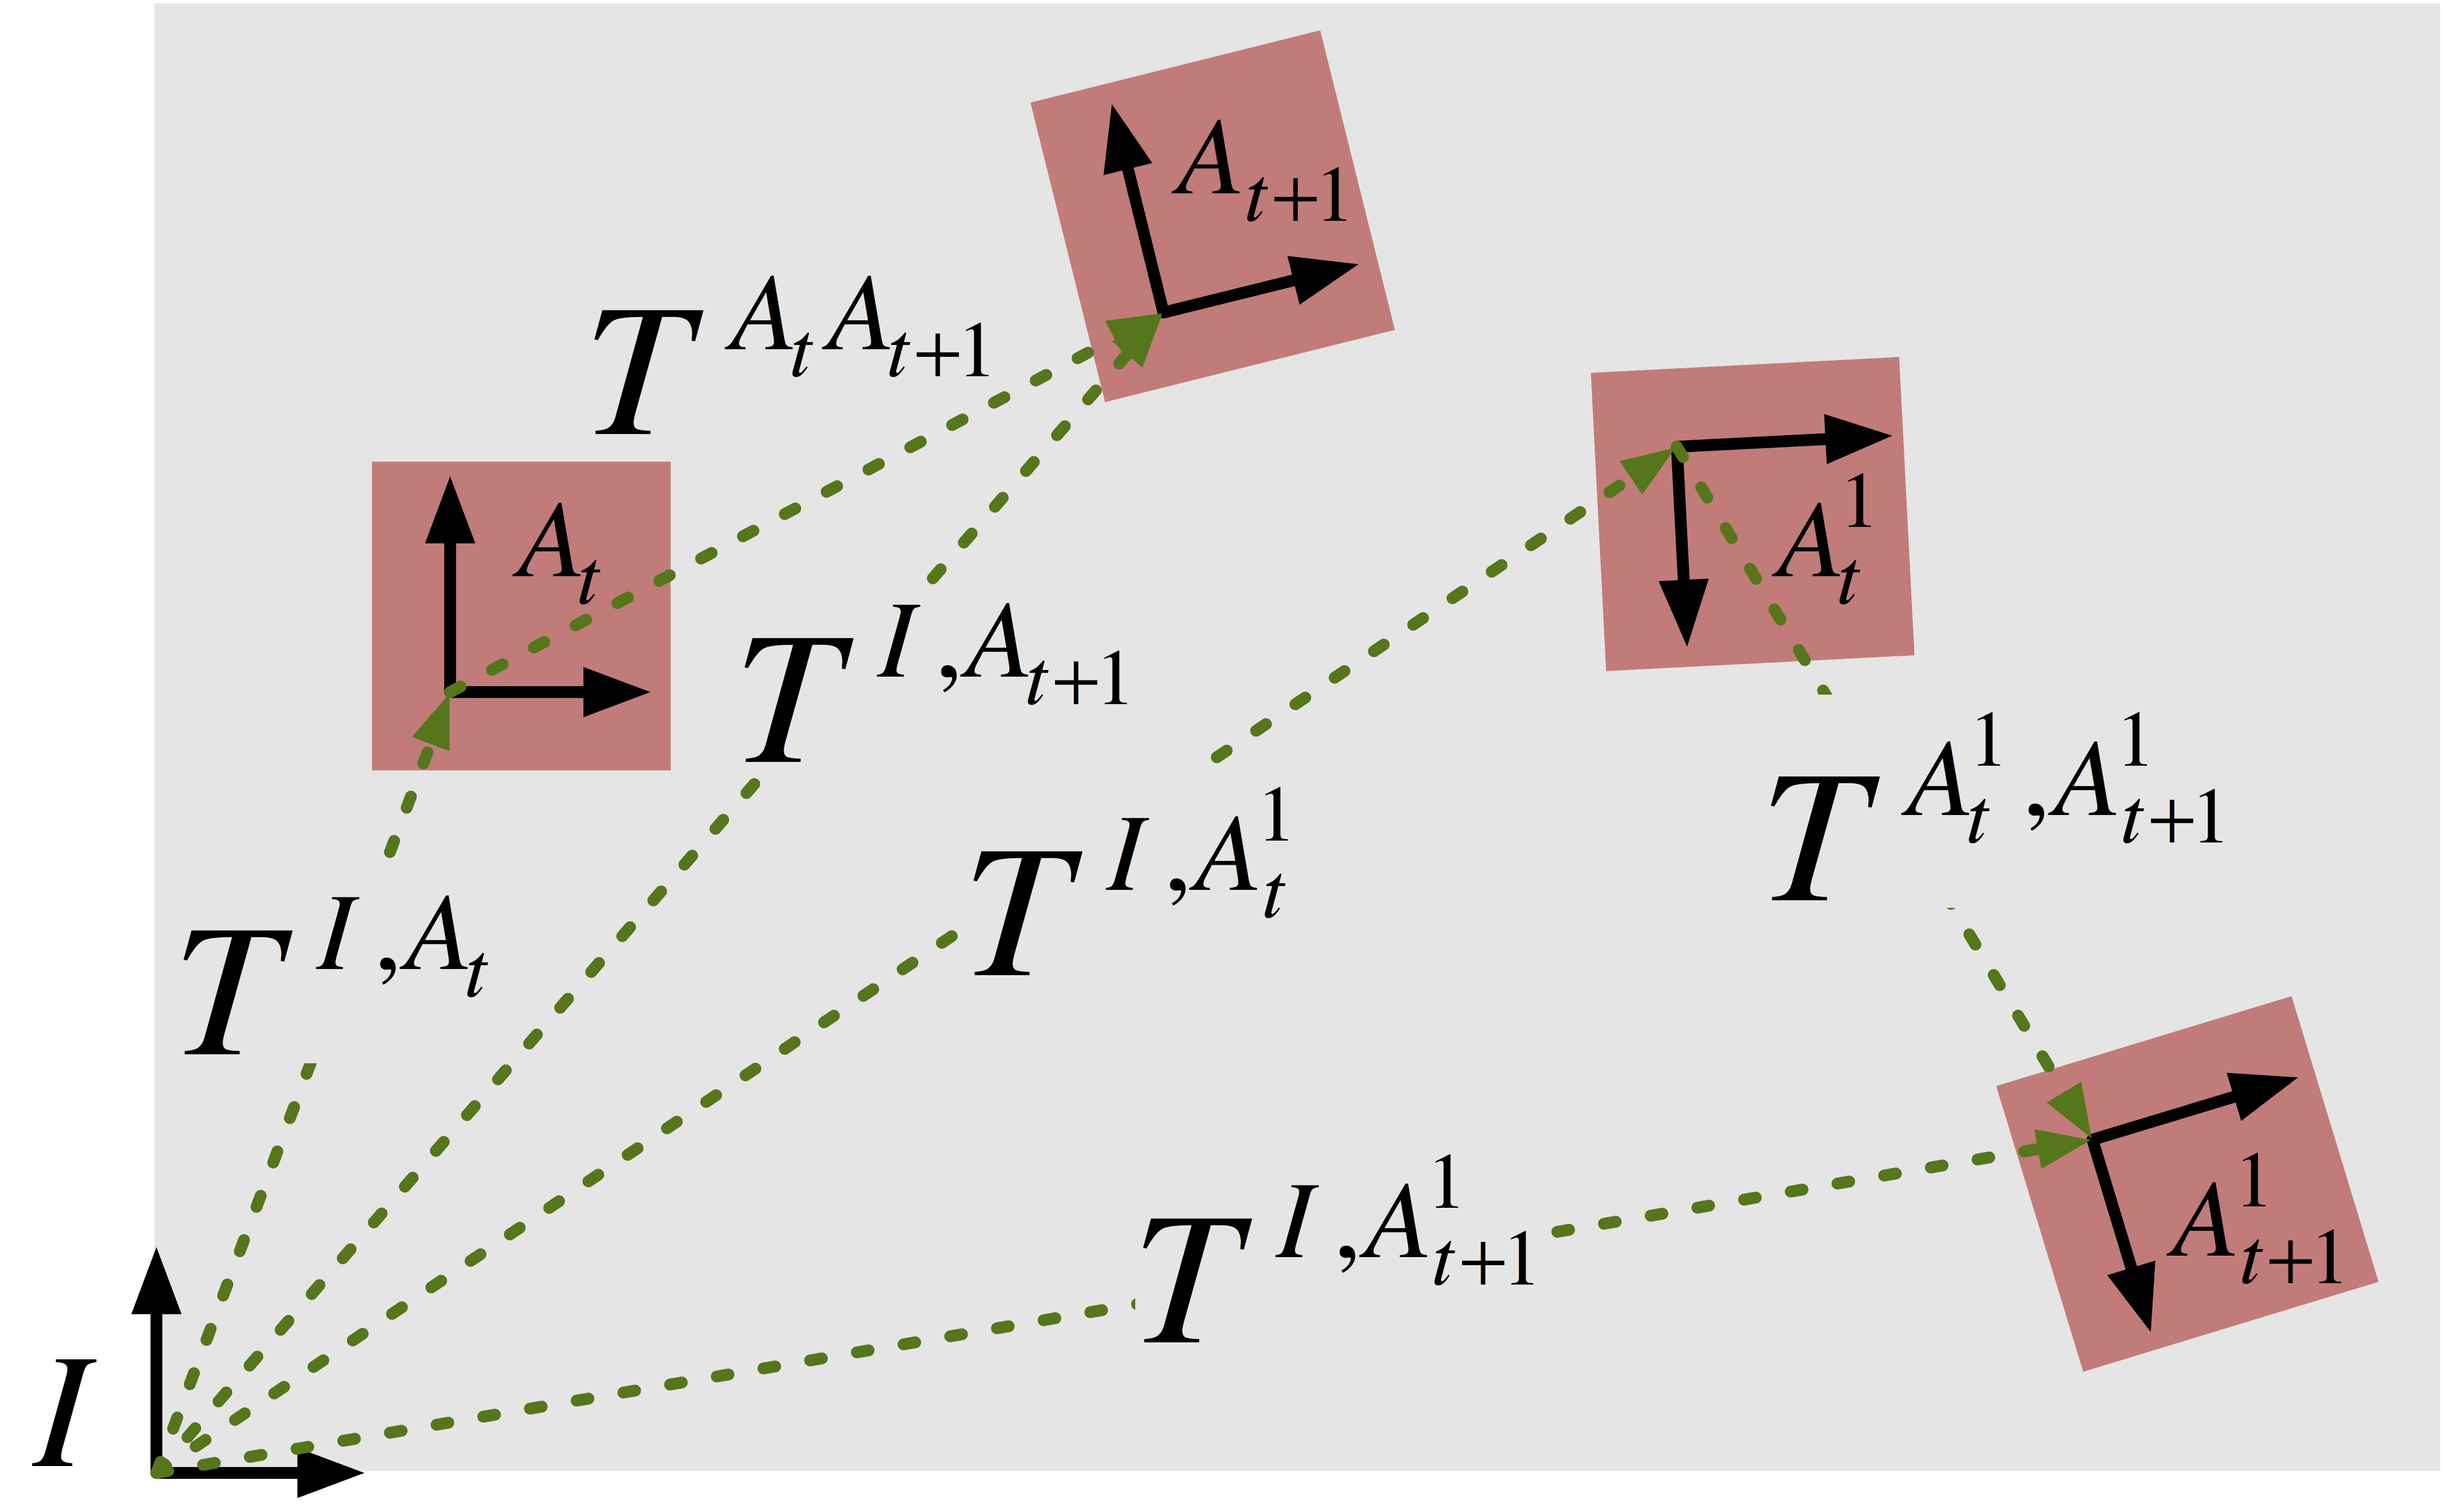
\includegraphics[width=\columnwidth]{similarity-new}}
%\caption[Similarity]{ Overhead view of an object on a table starting in two different positions. In each case the motion from $t$ to $t+1$ is the same relative to the instantaneous object body frames $A$ and $A^{1}$. However because transformations $T^{I, A}$ and $T^{I, A^{1}}$ are different, the corresponding transformations in the inertial frame are also different, i.e.\ $T_{in}^{A_{t}, A_{t+1}} \neq T_{in}^{A^{1}_{t}, A^{1}_{t+1}}$.}
%\label{fig:similarity}
%\end{figure}
%Intuitively these similarity transforms align the inertial and body frames, perform the required transformation and then invert the transformation required to align them. In this manner, given the instantaneous object frame $A_{t}$ at time $t$, and the inertial frame dependent transformation
%$T_{in}^{A_{t}, A_{t+1}}$, one can obtain the body frame dependent
%transformation $T_{body}^{A_{t}, A_{t+1}}$:
%\begin{equation}
%T_{body}^{A_{t}, A_{t+1}} = (T^{I, A_{t}})^{-1} T_{in}^{A_{t}, A_{t+1}} T^{I, A_{t}}
%\label{eq:Learning.Body1}
%\end{equation}
%\noindent where $T^{I, A_{t+1}} =$ $T_{in}^{A_{t}, A_{t+1}} T^{I, A_{t}} =$ $T^{I, A_{t}} T_{body}^{A_{t}, A_{t+1}}$.
%
%It is this body frame dependent transformation that will be stored during learning. Conversely, when a prediction is required, given a body frame dependent transformation, the object
%frame $A_{t}$, and using Equation~\eqref{eq:Learning.Body1}, the
%inertial frame dependent transformation $T_{in}^{A_{t}, A_{t+1}}$ is
%recovered using:
%\begin{equation}
%T_{in}^{A_{t}, A_{t+1}} = T^{I, A_{t}} T_{body}^{A_{t}, A_{t+1}} (T^{I, A_{t}})^{-1}
%\label{eq:Learning.Body2}
%\end{equation}
This technique is critical to generalisation across inertial frames. In the rest of the paper we will retain subscripts $in$, but suppress subscripts $body$. Thus all transformations denoted $T^{X, Y}$ are transformations in the body frame $X$, related to the equivalent transform in some inertial frame using a similarity transform:
\begin{equation}
T^{X, Y} \equiv T_{body}^{X, Y} = ({T^{I, X}})^{-1} T_{in}^{X, Y} {T^{I, X}}
\label{eq:Learning.Similarity}
\end{equation}

\section{Formal statement: learning to predict}
\label{sec:PredictionProblem}

We now have the basics required to formally describe the one-step and then the multi-step prediction
problem in such a way that they become problems of learning to predict, and we can effectively tackle problem P1 (Action Interpolation).

\subsection{One step prediction} The one step prediction problem is formulated as follows. Given observations of the recent poses of the finger and object, and the planned motion of the finger, $T^{A_{t},  A_{t+1}}$, predict the resulting immediate motion of the object,
$T^{B_{t}, B_{t+1}}$.  This is a problem of finding a function~$f$:
\begin{multline}
f:T^{A_t, B_t}, T^{B_t, O}, T^{A_{t-1}, A_{t}}, T^{B_{t-1}, B_{t}}, T^{A_{t}, A_{t+1}} \\ \longrightarrow T^{B_{t}, B_{t+1}}
\label{eq:Learning.long}
\end{multline}

The function $f$ is capable of describing the effects of interactions between rigid bodies $A$ and $B$, provided that their physical properties and net forces are constant
in time,\footnote{A dynamic formulation could explicitly incorporate
net forces into the domain and codomain of \eqref{eq:Learning.long}.}
in the limit of infinitesimally small time steps.
Furthermore, it can be approximately learned from observations,
for some small fixed time interval $\Delta t$ between time steps.

If robotic manipulations are performed slowly we can assume quasi-static conditions, and ignore all frames at time $t-1$.  This conveniently reduces the dimensionality of the problem, giving a simplified function~$f_{qs}$:
\begin{multline}
f_{qs}: T^{A_t, B_t}, T^{B_t, O}, T^{A_{t}, A_{t+1}} \longrightarrow T^{B_{t}, B_{t+1}}
\label{eq:Learning.short}
\end{multline}

It is this quasi-static formulation that is used to train and test the learning methods in this paper.

\subsection{Multi-step prediction} Having stated the one-step prediction problem it is possible to solve the multi-step prediction problem.\footnote{In this paper we study the multi-step problem in all our experiments. While the single step problem has been studied for other time series its utility for manipulation planning is low. Second, given fine grained single step predictions it is very hard to distinguish prediction quality over a single step.} Given a predictor (either $f$ or
$f_{qs}$), the initial states of the finger, $T^{A_{1}, O}$, and object, 
$T^{B_{1}, O}$, and knowing the trajectory of the finger $A_{1},
\ldots A_{T}$ over $T$ time steps, one can predict the complete
trajectory of the object $B_{1}, \ldots B_{T}$, by simply iterating
the predictions obtained from $f_{qs}$.  So, the output of the
predictor at time~$t$ is used as the input to the predictor for the
next time step (Figure~\ref{fig:modular-simple}). While this is a well known approach, it is difficult to produce a predictor that will behave well over many time steps. Over time all predictors will diverge from reality. Thus, an empirical question is whether, for a particular domain and prediction scheme, predictions are reasonably close to reality, over a suitable number of steps. It is this multi-step prediction problem that is solved in this paper.
\begin{figure}[t]
\centerline{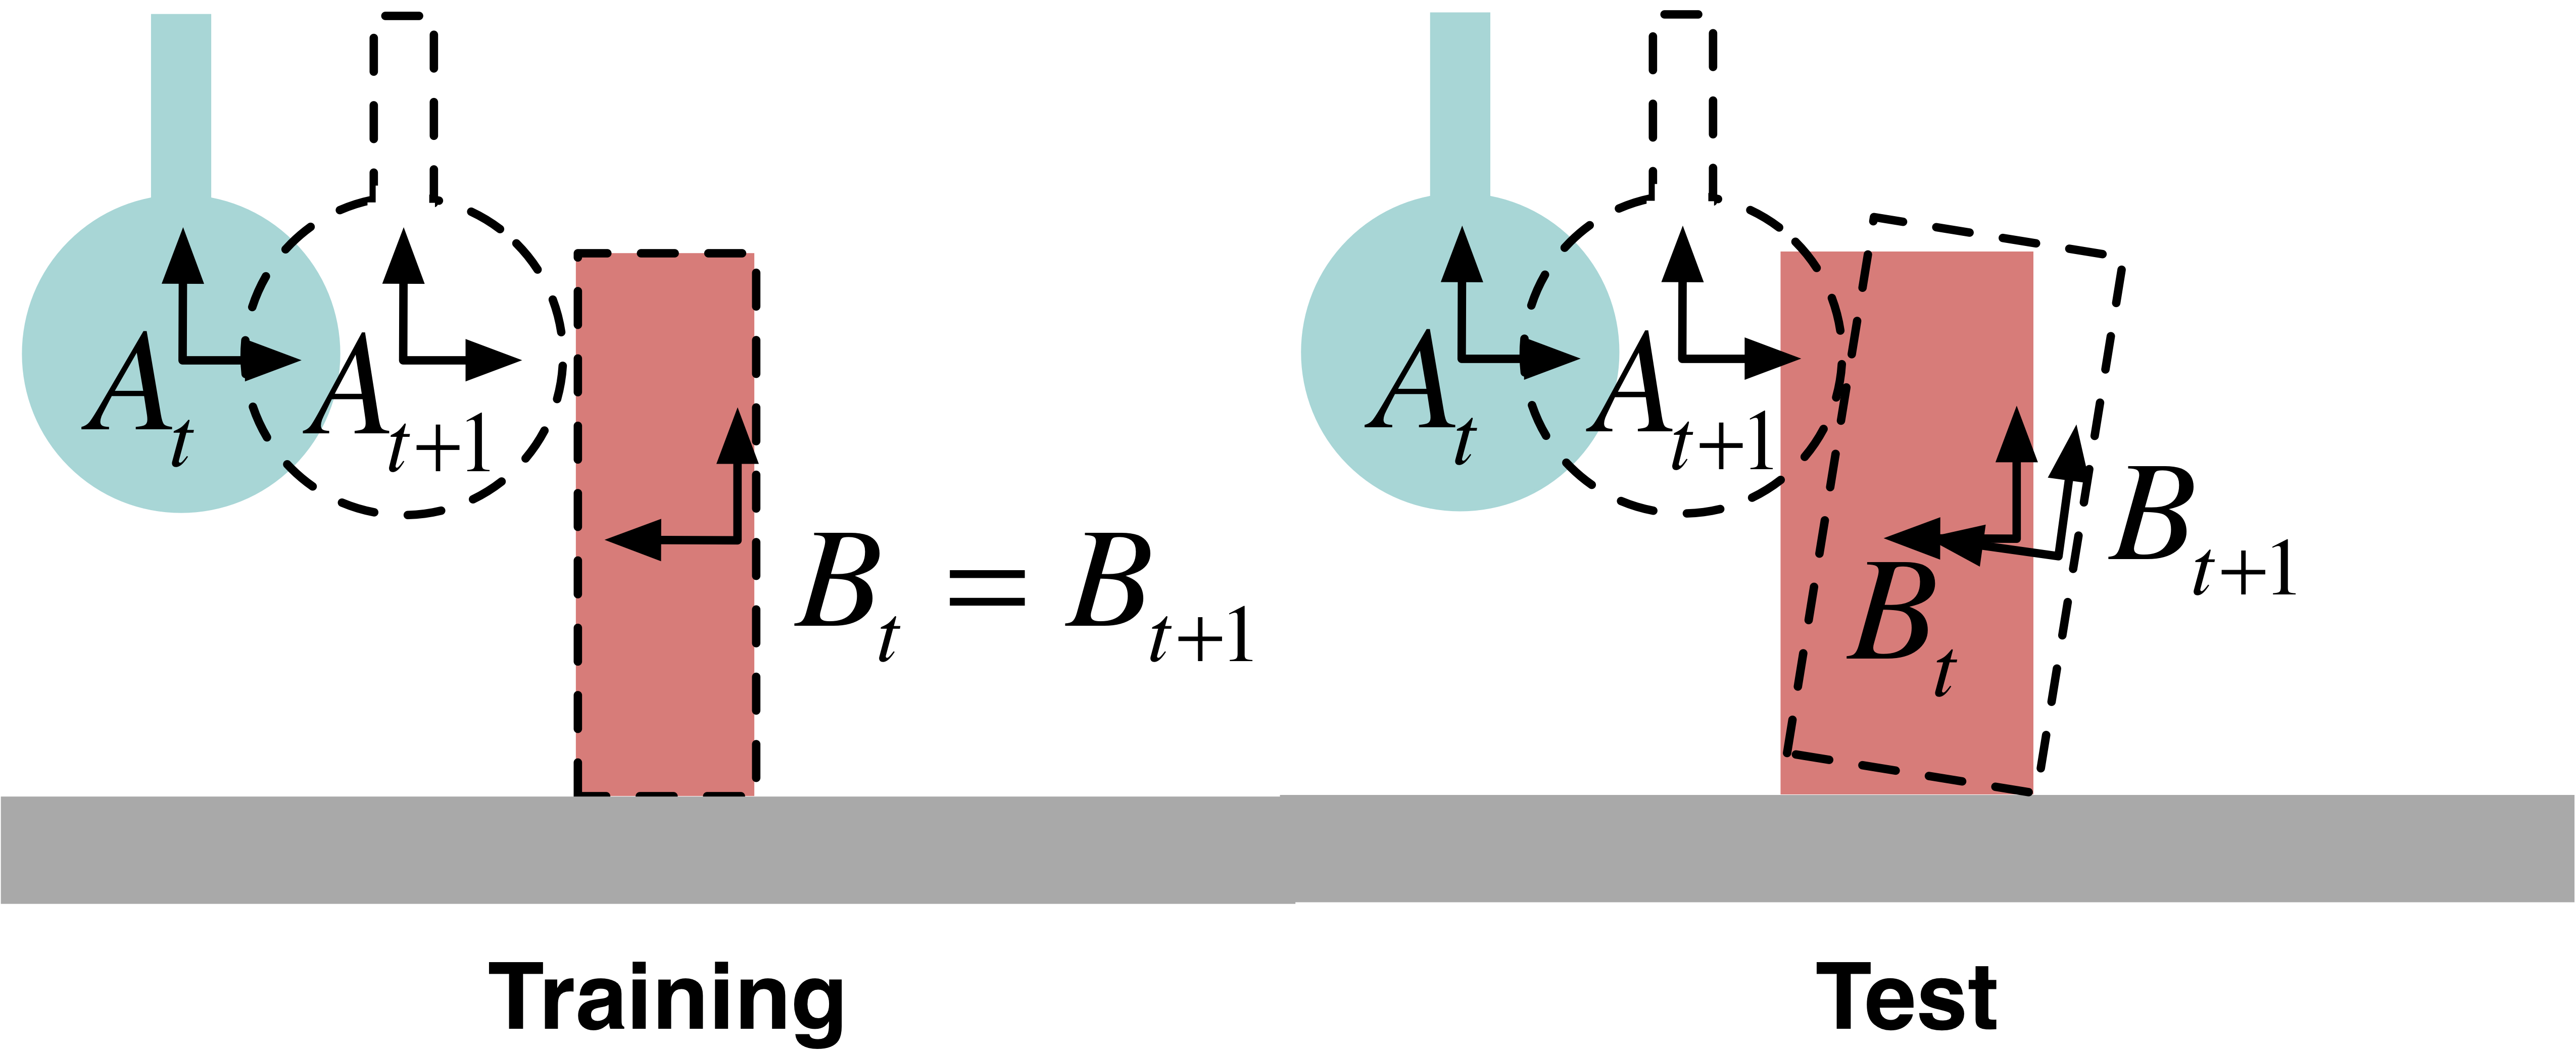
\includegraphics[width=\columnwidth]{shapes-colour}}
\caption[Shapes]{Two scenes (left and right),
each with an object on a tabletop. Only the shape of object $B$ differs between the scenes. Yet, when finger A moves, as shown by the dashed outline at time $t+1$, the resulting transformation of $B$ will be quite different.}
\label{fig:Learning.shapes}
\end{figure}
\subsection{Learning to predict as regression} In principle it is straightforward to acquire a predictor, $f$ or
$f_{qs}$, by learning it from data. Given sufficient experience of
object and finger trajectories, we can perform a nonparametric
regression analysis, by taking $T^{A_t, B_t}$, $T^{B_t, O}, T^{A_{t},
  A_{t+1}}$ as independent variables, and $T^{B_{t}, B_{t+1}}$
as the dependent variable.  Nonetheless, a powerful regression
technique is needed, since the domain of $f_{qs}$ has 18~dimensions
or more, depending on the parameterisation of motion.
\begin{figure*}[t]
\centerline{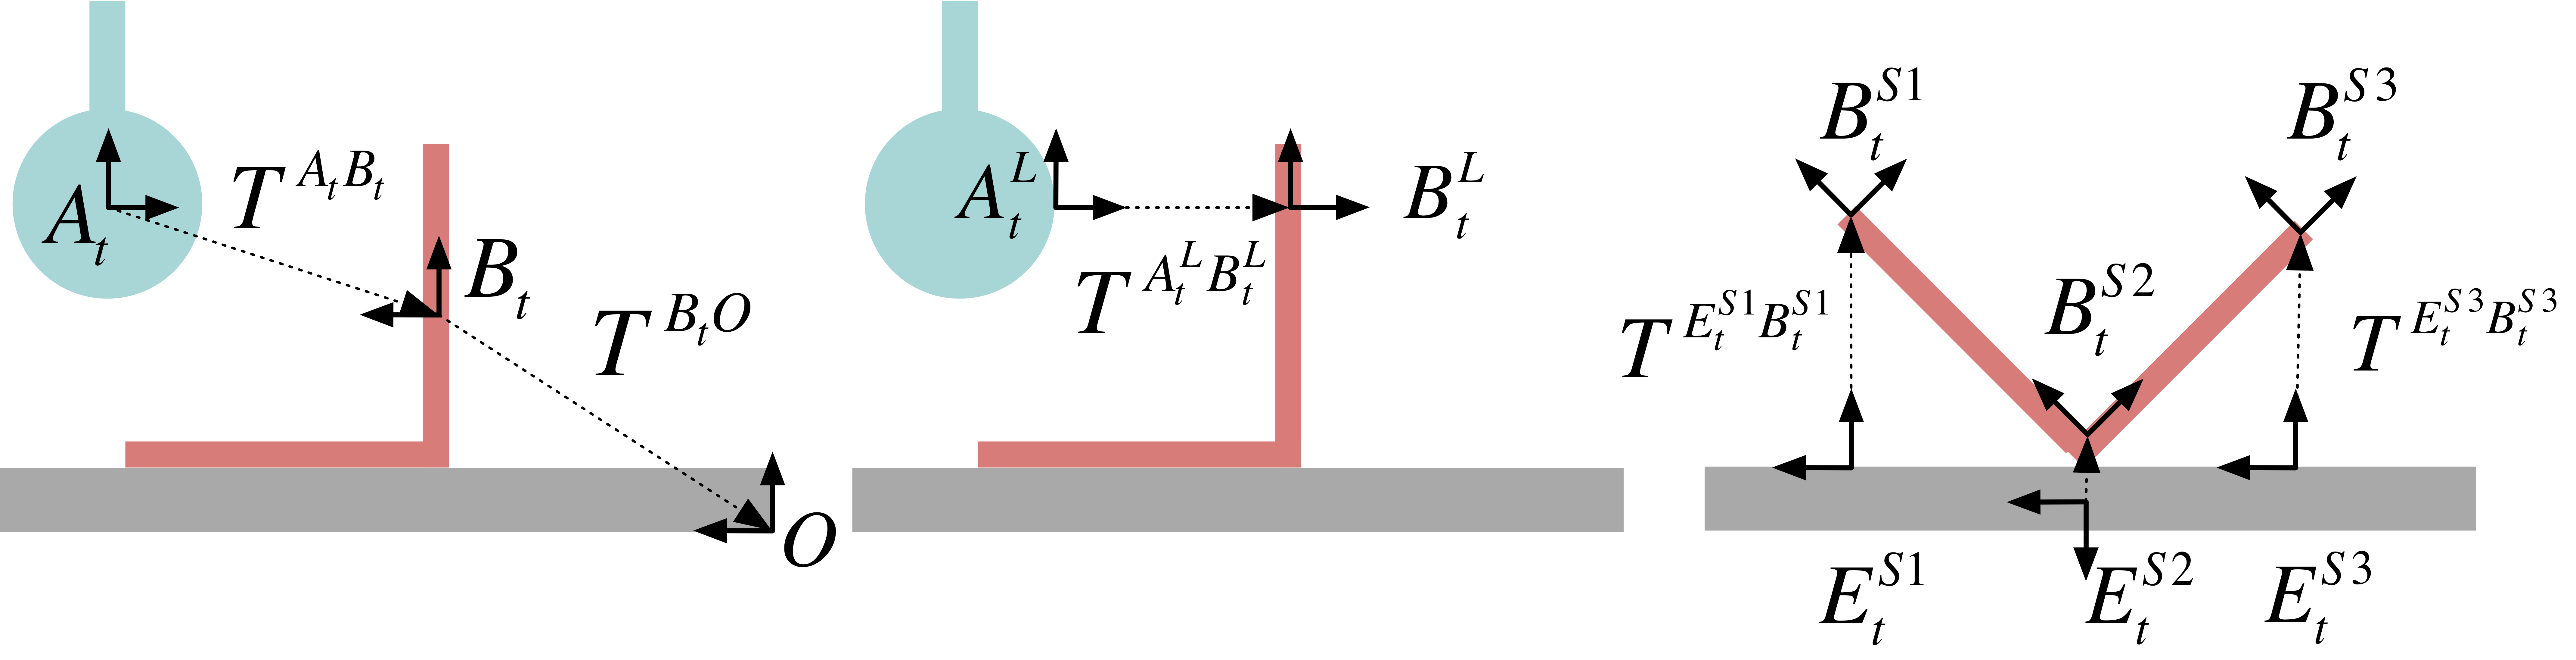
\includegraphics[width=\textwidth]{information}}
\caption{Three types of information useful in prediction problems. Left: (G - global) global frames of reference for the robot, object and the world. Centre: (A - agent) local frames of reference on the robot finger and the closest point on the object. Right (E - environment) local frames of reference on the object and the closest points on surfaces in the environment.}
\label{fig:Learning.setup2}
\end{figure*}
\subsection{Learning to predict as density estimation} As an alternative to learning the mapping~\eqref{eq:Learning.short} by regression, we can recast $f_{qs}$ as a conditional probability density (CPD) $p_{qs}$ over possible object motions $T^{B_{t},B_{t+1}}$ \citep{kopicki_prediction_2009}:
\begin{equation}
p_{qs}(T^{B_{t}, B_{t+1}} | T^{A_t, B_t}, T^{B_t, O}, T^{A_{t}, A_{t+1}})
\label{eq:Learning.density1}
\end{equation}

The learning problem is then posed as one of density estimation. This permits modelling the probabilities of many possible outcomes. 

Either the regression or density estimation formulation can be used in a modular scheme. In this case a separate module is learned for each combination of agent, object, and environment. Each module interpolates over actions for its context, and thus the overall system solves problem P1. We now identify the additional information needed to solve problems P2 and P3.


\section{Transfer Learning}
\label{sec:InfoForPrediction}

\subsection{The need for contact models}
The input domains of $f$, $f_{qs}$, and $p_{qs}$ are insufficient to pose problems P2 (Action Transfer) or P3 (Shape Transfer). This is because they only capture the {\em global} relations between objects. To properly pose transfer learning, the input domain must capture all the {\em local} contact relations between the object and its surroundings.  To see why consider Figure~\ref{fig:Learning.shapes}. On the left is a training example. On the right is a test case, where the object is wider. Given the same placement of the frames on object and agent, and the same finger motion, the predicted behaviour using Equation~\eqref{eq:Learning.short} will be the same as for the training example. This is wrong. For the correct prediction to be transferred, additional information is needed about the contact between $A$ and $B$. This can be captured by attaching additional frames to $A$ and $B$  (Figure~\ref{fig:Learning.setup2}). In general, an object has multiple contacts with the robot and the environment. Each of these contacts provides a kinematic constraint on the object's motion, and thus each one should be modelled. Rigid body simulators use just such contact information.

\subsection{Modelling contacts and near contacts} 
We use a pair of local frames to encode each contact or near contact. Each pair encodes a transformation between part of the object $B$ and another body.  To distinguish these local frame pairs from what has gone before we henceforth refer to the main frame attached to a body (defined in Section~\ref{sec:Representations}) as that body's global frame. We define the local frame pairs as follows. Consider Figure~\ref{fig:Learning.setup2}. We first define a pair of local frames capturing the finger-object contact as $A^{L}_{t}$ and $B^{L}_{t}$ (centre panel). These are spatially dynamic, i.e.\ at any time $t$ they are located at the points of closest proximity on the finger and object respectively.  We define the \textit{agent-object contact}
information as the transformations $T^{A^{L}_{t}, A^{L}_{t+1}}$ and $T^{A^{L}_t, B^{L}_t}$.

We also define local frame pairs, to model object-environment contacts. One frame is attached to some point on the object ($B^{Sk}_t$), and one is attached to the nearest point in the environment $E^{Sk}_t$.  Thus the environment frame within each pair is spatially dynamic, changing its position as the object moves. If $N$ points on the object are chosen for modelling there will be $N$ pairs of local frames $B^{Sk}_t$ and $E^{Sk}_t$ to capture the object-environment contacts at time $t$, where ($k=1 \ldots N$) (Figure~\ref{fig:Learning.setup2} right panel). Using these frame pairs, we then define the \textit{object-environment contact} information as the set of transformations $T^{E^{Sk}_t,B^{Sk}_t}$ for $k=1 \ldots N$. 

This section described the information required to allow transfer learning. We refer to this as {\em contact} information, even though it also includes information on surfaces not in, but close to, contact. 

\subsection{Learning a contact model}
Given observations of moving surfaces in contact, and near contact, it is possible to learn contact models. In this paper, during training, two contact models are learned: an agent-object contact model, and an object-environment contact model. The object-environment contact model is created by pooling data from frames located at several points on the object. Thus, a learned model of contact behaviour is created from many contact examples. This contrasts with the analytic approach used by rigid body simulators. An extension would be to condition this model on other variables, for example information on local surface properties, such as shape or texture. We hypothesize that both data pooling and conditioning will be important elements in improving the transfer of predictions. 

\begin{figure}[t]
\centerline{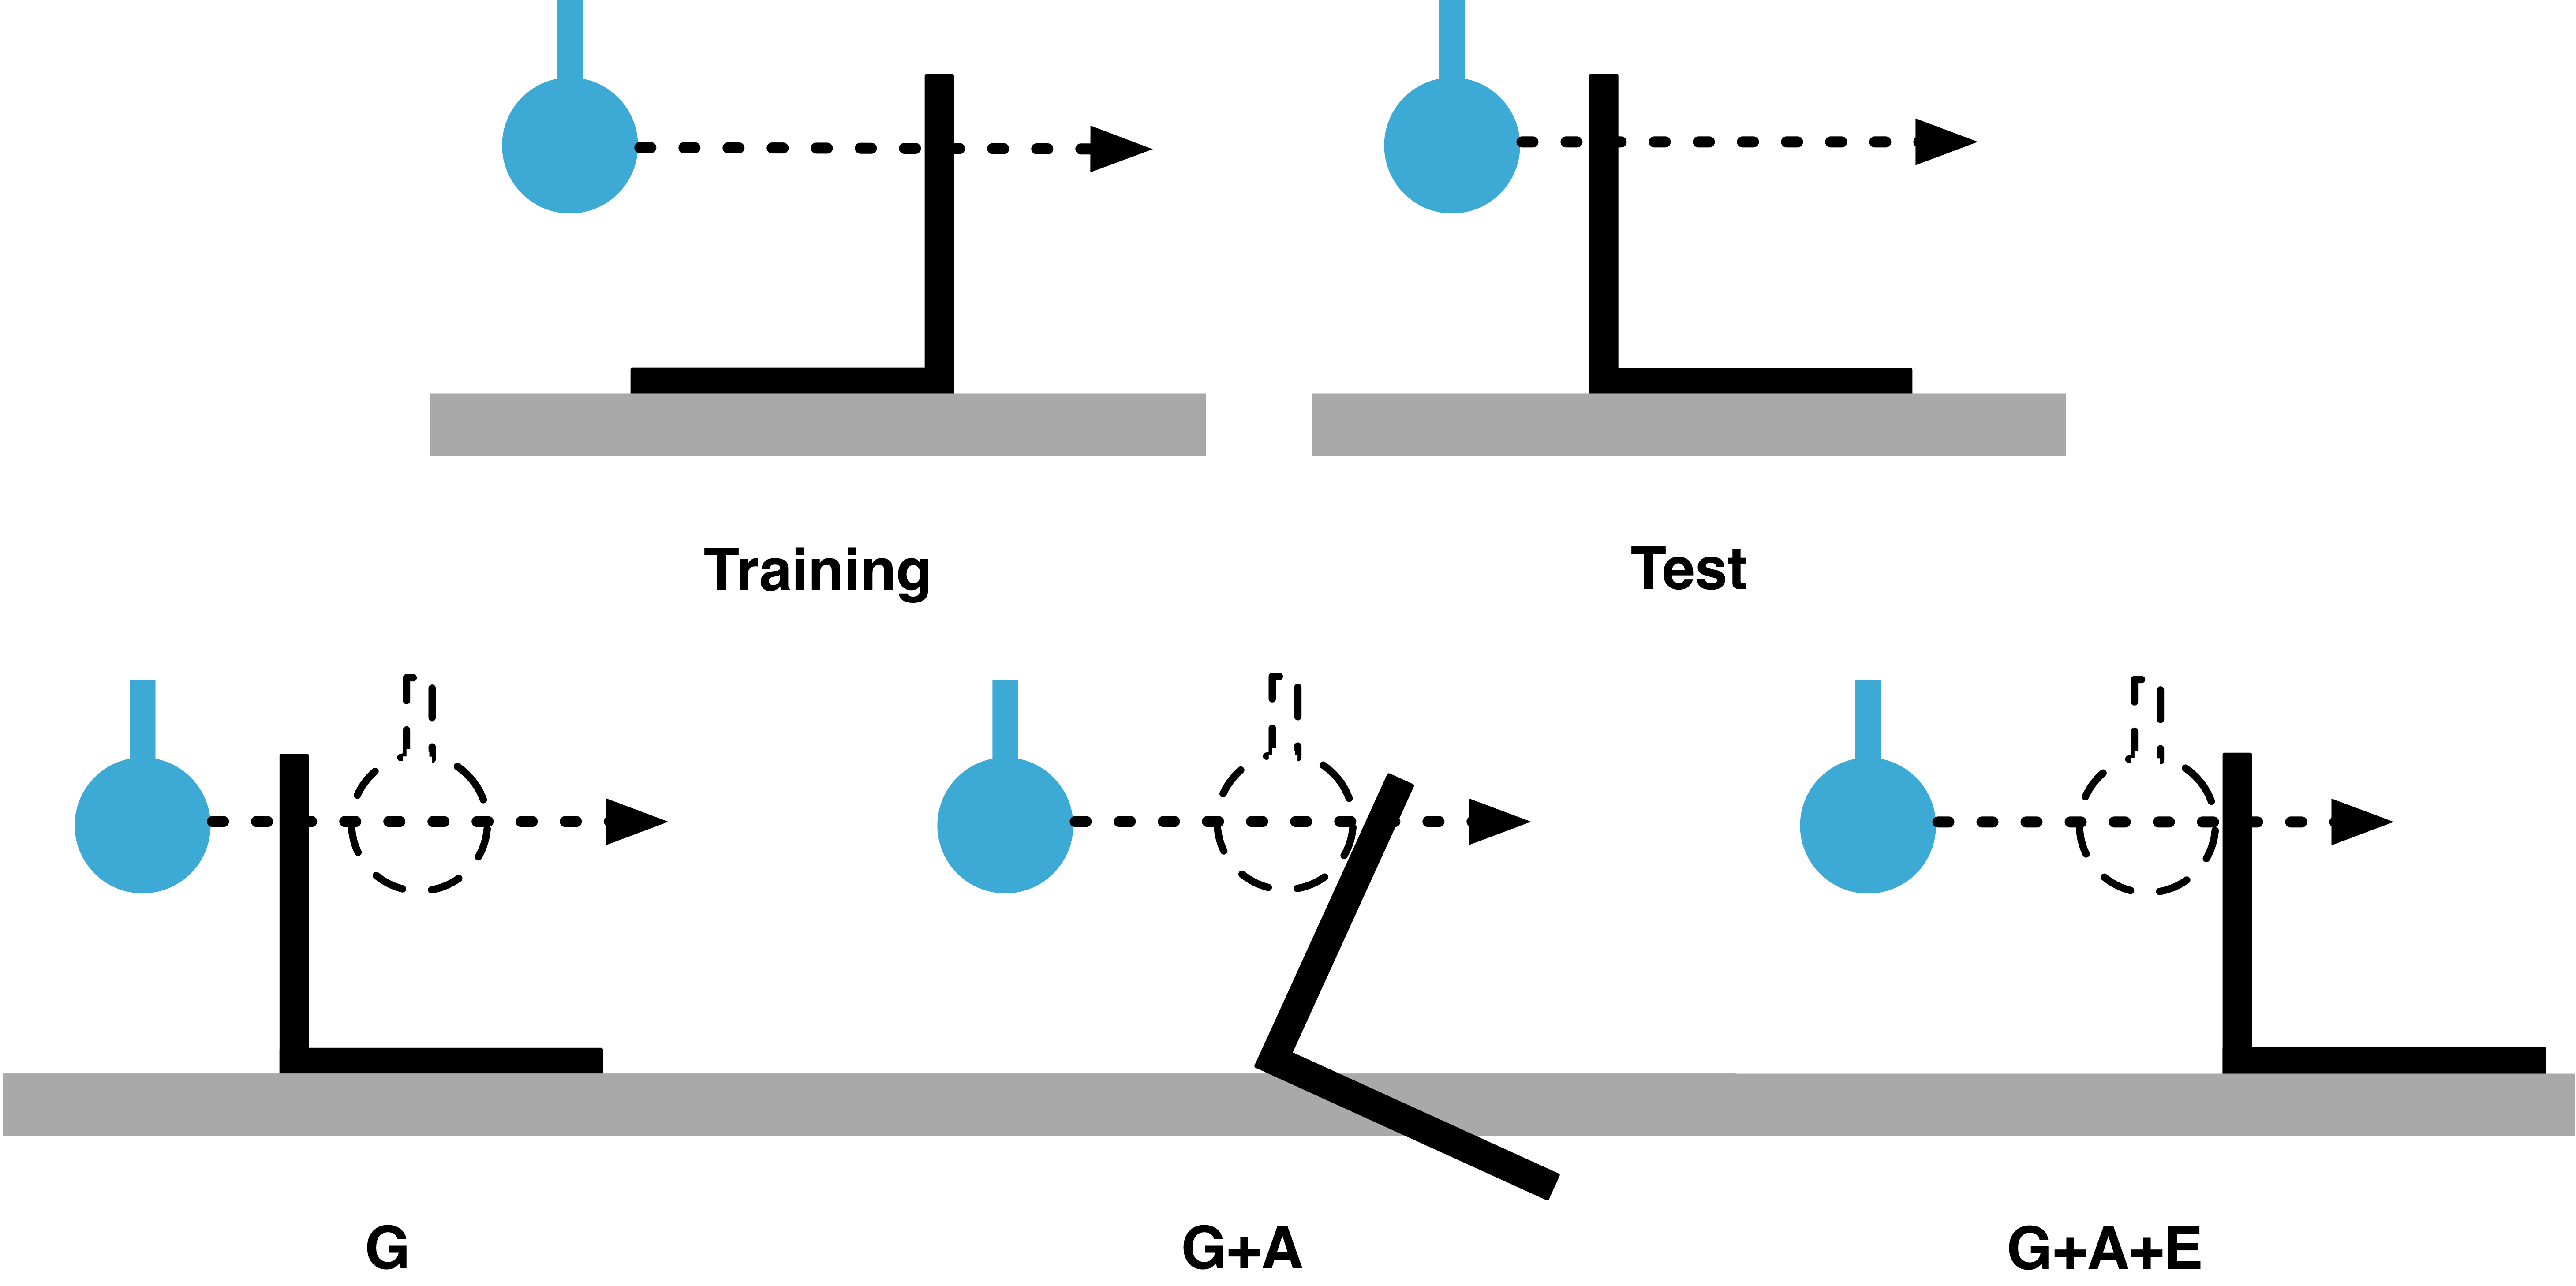
\includegraphics[width=\columnwidth]{BackPushToyExample}}
\caption[ToyExample]{Information for Action Transfer: an L-shaped object is pushed by a finger. Various predictors are trained solely on forward pushes (top left), but tested on backwards pushes (top right). The top panels show a training and a test push, whereas the bottom panels show predictions given different information (G, G+A and G+A+E) for the test push.}
\label{fig:ToyExample}
\end{figure}

\subsection{Predicting with contact models}
During prediction the learned contact models are applied to the test case. This requires mapping the various reference frames from the training examples to the test examples. For problems P1 and P2 this is trivial, since the objects are the same. For problem P3 the placement can be made in several ways. In our implementation we used heuristic rules. The global frame was attached to the most central point lying within the object. The agent-object frames were automatically attached, each step, to the object location closest to the finger. Finally, $N$ object-environment frames, $B^{Sk}_t$, were attached to points on the object surface with curvature sufficiently similar to that in the training data which contributed to the contact model. This heuristic strategy was empirically determined to be robust. Because of data pooling during training, each object-environment expert is a copy of a single object-environment model. Thus several, identical, contact experts are created on the new object. Other ways to automate the placement strategy for P3 are possible. 

Finally, we note that we have motivated these contact experts as enabling shape transfer, but they are equally applicable to action transfer. The top row of Figure~\ref{fig:ToyExample} shows a training and a test case for problem P2 (action transfer). The prediction for the test case requires encoding of the kinematic constraint imposed by the contact between the base of the L-shaped flap and the table. This constraint also existed in the training push, but was not significant since the flap could rotate on its corner.

\subsection{Hypothesized benefits of contact modelling}
We can now consider the effects that different sets of information might have. We shall refer to a predictor that uses only the global frames, $A$ and $B$, as having global information (G). We can add agent-object contact information (G+A), and object-environment contact information (G+A+E). Now consider the possible predictions for the test case (Figure~\ref{fig:ToyExample} bottom row). A predictor using G will predict that the object will not move. A predictor using G+A has information, from the training case, that the object surface will move with the finger, so that the finger will not pass through it. But this information is also capable of predicting that the object rotates about the corner and into the table, since it doesn't model the object-environment contact. A predictor using G+A+E will have information about the effect of the contact between the base of the flap and the table, and so should avoid predicting a rotation into the table.
One point is critical, this analysis only concerns what the information allows. Performance will depend on a learner's ability to utilise it.  

\subsection{Reformulating prediction with contact information}
We can simply extend the prediction formulations to incorporate contact information. For regression we simply enlarge the domain of function~$f$
in Equation~\eqref{eq:Learning.short}:
\begin{multline}
f'_{qs}: T^{A_t, B_t}, T^{B_t, O}, T^{A_{t}, A_{t+1}}, T^{A^{L}_t, B^{L}_t} \\ \{, T^{E^{Sk}_t,B^{Sk}_t}\}_{k=1 \ldots N} \longrightarrow T^{B_{t}, B_{t+1}}
\label{eq:Learning.augmented}
\end{multline}
Recall that, at prediction time, we will need $N$ copies of the object-environment contact information, which was pooled at the learning stage. Hence, we use $k$ to index over these copies. Unfortunately, because the dimensionality of the domain of $f'_{qs}$ grows with the number of environment contacts, $N$, the difficulty of learning the mapping $f'_{qs}$ rapidly increases as environment contacts are added.

The conditional probability density (CPD) $p_{qs}$ over possible object motions $T^{B_{t}, B_{t+1}}$~\citep{kopicki_prediction_2009} is augmented as follows:
\begin{multline}
p_{qs}(T^{B_{t}, B_{t+1}} | T^{A_t, B_t}, T^{B_t, O}, T^{A_{t}, A_{t+1}}, T^{A^{L}_t, B^{L}_t} \\ \{, T^{E^{Sk}_t,B^{Sk}_t}\}_{k=1 \ldots N})
\label{eq:Learning.density}
\end{multline}

Again, the dimensionality of the conditioning variables makes density estimation hard as the number of contacts grows. One way around this, in the density estimation case, is to factorize the density in a way that reflects the contact structure. We consider this in the next section.

\section{Factorised density estimation}
\label{sec:Factors}

Both formulations give learning problems that increase in difficulty as further contacts are added. One question is whether either formulation can be recast, so as to take advantage of the natural
problem structure. This section presents one such scheme for the
density estimation (or CPD) formulation, based on a product of experts (Figure~\ref{fig:modular}).

Specifically, the CPD formulation allows us to factorise the density,
and approximate $p_{qs}$, by making a conditional independence
assumption. The unfactored CPD formulation gives a density over
possible one step motions of the object. We can
factorise this by breaking up the conditioning variables into groups,
according to the contacts. This reflects the notion that the behaviour
at each contact is independent of the other contacts. Each component of the product is an expert, which encodes the likely object motions given a single kinematic constraint. The product will be maximised by a motion that best satisfies all the constraints simultaneously.

The computational advantage is that, since the component
densities factorise the conditioning variables of $p_{qs}$, the overall predictor works better with a high dimensional input space.  Furthermore, the subset of experts used in the product can be selected dynamically, depending on the current set of contacts. For some normalisation constant~$C$ we propose the following factorisation:
\begin{equation}
p_{qs} \approx C\ p_{global}\ p_{agent}\ \mathop{\prod}_{k=1 \ldots N}{ p_{env,k}}
\label{eq:Learning.product}
\end{equation}
\noindent where
\begin{subequations}
\begin{align}
p_{global} &\equiv p_{global}(T^{B_{t}, B_{t+1}}|T^{A_{t}, A_{t+1}}, T^{A_t, B_t}, T^{B_t, O})
\label{eq:Learning.densityglobal} \\
p_{agent} &\equiv p_{agent}(T^{B^{L}_{t}, B^{L}_{t+1}}|T^{A^{L}_{t}, A^{L}_{t+1}}, T^{A^{L}_t, B^{L}_t})
\label{eq:Learning.densitylocal} \\
p_{env,k} &\equiv p_{env,k}(T^{B^{Sk}_t, B^{Sk}_{t+1}} | T^{E^{Sk}_t,B^{Sk}_t})
\label{eq:Learning.densityenv}
\end{align}
\end{subequations}

\noindent denote the \textit{global}, \textit{agent-object}, and
$k^{th}$ \textit{object environment} density factors,
respectively~\citep{kopicki_prediction_2009, kopicki_prediction_2010}. 
The one step prediction problem can then be defined as finding the
transformation $\widetilde{T}_{in}^{B_{t}, B_{t+1}}$, expressed in some inertial frame, which maximises the product of densities \eqref{eq:Learning.product}:
\begin{equation}
\widetilde{T}_{in}^{B_{t}, B_{t+1}} = \argmax{T_{in}^{B_{t}, B_{t+1}}} \bigg\lbrace
p_{global}\  p_{agent} \mathop{\prod}_{k=1 \ldots N}{ p_{env,k} }
\bigg\rbrace
\label{eq:Learning.MultiFactorProduct}
\end{equation}

\noindent where similarity transforms, as described in Section~\ref{sec:Representations}, must be used to evaluate $p_{global}$, $p_{agent}$, and the $N$ environment factors $p_{env,k}$, for a given ${T}_{in}^{B_{t}, B_{t+1}}$.
\begin{figure}[t]
\centerline{\includegraphics[width=\columnwidth]{product-predictor}}
\caption[Factored Prediction]{A Dynamic Product of Experts. This gives the structure of a factorised predictor for a single context, as depicted in the modular learner in Figure~\ref{fig:modular-simple}. Each expert in the product has an applicability condition, which determines whether it contributes to the product. The applicable predictors combine densities over predictions to produce an overall density. This is optimised to produce a specific prediction.}
\label{fig:modular}
\end{figure}

The key property here is that the global, agent, and environment densities encode different information as to which rigid body transformations are feasible. By taking the product of these densities, only transformations which are feasible in all factors' frames will have high probability in the resulting combined distribution. In addition, we make this product dynamic in the number of object-environment factors. Once the object surface is above some threshold distance from the environment surface its predictor switches off, and when it is close enough it switches on again. This enables us to keep only relevant predictors in the product at any one time -- improving prediction quality and efficiency. 

In summary, we have now described two main formulations (regression and density estimation) able to incorporate varying amounts of information (G, G+A, G+A+E). We have also presented a reformulation of density estimation that factorises the prediction problem, given information G+A or G+A+E, into a product of experts. Which information and problem formulation should be combined to provide the best prediction framework?
Is the factorised problem better able to exploit the additional
information than the unfactorised version? These questions can only be
answered using specific regression and density estimation
algorithms. Having completed our problem formulation we therefore now
turn to the details of the implementations for each framework.
